\chapter{Architecture}
\label{chap:arch}
\thispagestyle{fancy}
\pagestyle{fancy}

Podemos dividir o sistema em 3 camadas principais. 


\section{Configuration Layer}
The Configuration Layer is responsible for representing, loading, and validating the deployment plan before any real-time activity begins. The deployment plan is a Json file that holds the specification of the aplication, that includes: all the task and subtasks and their component type, the connections between the subtasks, which host and core the subtask should be executed.
A Figura \ref{fig:config_layer} mostra o caminho de execução do configuration layer, começando do arquivo json lido e traduzido para variáveis da aplicação e termina na população da estrutura de dados DAG a partir das conexões de predeceção e sucessão.


  \begin{figure}[htbp]
  \centering
  \resizebox{\textwidth}{!}{%
  \begin{tikzpicture}[
    >=Stealth, thick,
    box/.style={
      draw, rounded corners=3pt, fill=blue!8, align=center,
      minimum height=0.8cm, minimum width=2.4cm, font=\small\ttfamily
    },
    arr/.style={->, semithick},
    lbl/.style={font=\scriptsize\sffamily, fill=white, inner sep=1.5pt}
  ]
  
    %% Nodes
    \node[box] (JSON) at (0,     0)     {deployment\_plan\\.json};
    \node[box] (JP)   at (3,     0)     {JsonParser\\::parse()};
    \node[box] (DP)   at (6,     0)     {DeploymentPlan};
    \node[box] (HI)   at (9,     1.5)   {HostInfo[]};
    \node[box] (TI)   at (9,     0)     {TaskInfo[]};
    \node[box] (CI)   at (9,    -1.5)   {ConnectionInfo[]};
    \node[box] (SI)   at (12,    0.75)  {SubtaskInfo[]};
    \node[box] (DAG)  at (14.5, -0.5)   {DAG};
    \node[box] (NODE) at (17.5, -0.5)   {DAG::Node[]};
    
    %% Edges
    \draw[arr] (JSON) --      (JP);
    \draw[arr] (JP)   --                                  (DP);
    \draw[arr] (DP)   --                                  (HI);
    \draw[arr] (DP)   --                                  (TI);
    \draw[arr] (DP)   --                                  (CI);
    \draw[arr] (TI)   --                                  (SI);
    \draw[arr] (SI)   -- node[lbl, above right]{add\_node()} (DAG);
    \draw[arr] (CI)   -- node[lbl, below right]{add\_edge()} (DAG);
    \draw[arr] (DAG)  --                                  (NODE);

    %% Subgraph border (Configuration Layer)
    \begin{scope}[on background layer]
      \node[
        draw=gray!70, dashed, rounded corners=8pt, fill=gray!5,
        inner sep=12pt,
        fit=(JSON)(JP)(DP)(HI)(TI)(CI)(SI)(DAG)(NODE),
        label={[font=\small\bfseries\sffamily, anchor=south]above:Configuration Layer}
      ] {};
    \end{scope}
  
  \end{tikzpicture}
  }
  \caption{Configuration layer from deployment plan to DAG construction.}
  \label{fig:config_layer}
  \end{figure}

The Figura \ref{fig:deployment_class} mostra o diagrama de classe de Deployment Plan, note que existe um HostInfo, que são as informações de conexão com outros computadores para uma futura expansão para um sistema distribuído.

\begin{figure}[htbp]
  \centering
  \resizebox{\textwidth}{!}{%
  \begin{tikzpicture}
  
    \begin{class}[text width=5.2cm]{DeploymentPlan}{4.5,12}
      \attribute{+ hosts : HostInfo{[]}}
      \attribute{+ tasks : TaskInfo{[]}}
      \attribute{+ connections : ConnectionInfo{[]}}
    \end{class}
    
    \begin{class}[text width=4cm]{HostInfo}{0,7}
      \attribute{+ name : string}
      \attribute{+ address : string}
    \end{class}
    
    \begin{class}[text width=4.5cm]{TaskInfo}{4.5,7}
      \attribute{+ id : int}
      \attribute{+ subtasks : SubtaskInfo{[]}}
    \end{class}
    
    \begin{class}[text width=4cm]{ConnectionInfo}{9.5,7}
      \attribute{+ upstream : int}
      \attribute{+ downstream : int}
    \end{class}
  
    \begin{class}[text width=5.5cm]{SubtaskInfo}{4.5,1}
      \attribute{+ task\_id : int}
      \attribute{+ id : int}
      \attribute{+ component\_type : string}
      \attribute{+ host : string}
      \attribute{+ core : int}
      \attribute{+ priority : int}
      \attribute{+ period\_ns : uint64}
      \attribute{+ deadline\_ns : uint64}
      \attribute{+ config : json} 
    \end{class}
    
    \composition{DeploymentPlan}{}{1}{HostInfo}{}{N}
    \composition{DeploymentPlan}{}{1}{TaskInfo}{}{N}
    \composition{DeploymentPlan}{}{1}{ConnectionInfo}{}{N}
    \composition{TaskInfo}{}{1}{SubtaskInfo}{}{N}

  \end{tikzpicture}
  }
  \caption{Class diagram of the DeploymentPlan data model.}
  \label{fig:deployment_class}
  \end{figure}




\section{Scheduling Layer}

The Scheduling Layer is the one that actualy executes the subtasks. Essa camada é composta apenas pelo arquivo Dispatcher, que é um componente presente em todo conjunto de subtasks pertencentes ao mesmo core com mesma  priority.
Each Dispatcher instance manages two concurrent threads pinned to the same CPU core, operating at different priority levels. The main thread runs at the assigned real-time priority and remains asleep until a subtask is ready for execution. Upon activation, it dequeues the pending subtask, enforces its release-time constraints, runs its computation, and automatically triggers all downstream subtasks before returning to the sleep state.



\tikzset{every picture/.style={line width=0.75pt}} %set default line width to 0.75pt        

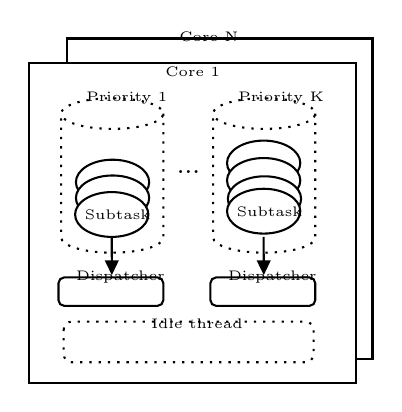
\begin{tikzpicture}[x=0.75pt,y=0.75pt,yscale=-1,xscale=1]
%uncomment if require: \path (0,274); %set diagram left start at 0, and has height of 274

%Shape: Rectangle [id:dp4242428752516575] 
\draw  [fill={rgb, 255:red, 255; green, 255; blue, 255 }  ,fill opacity=1 ] (63.66,35.11) -- (210.91,35.11) -- (210.91,189.51) -- (63.66,189.51) -- cycle ;
%Shape: Rectangle [id:dp20915950450837784] 
\draw  [fill={rgb, 255:red, 255; green, 255; blue, 255 }  ,fill opacity=1 ] (45.26,47.11) -- (202.91,47.11) -- (202.91,201.11) -- (45.26,201.11) -- cycle ;
%Shape: Ellipse [id:dp09636426316005864] 
\draw  [fill={rgb, 255:red, 255; green, 255; blue, 255 }  ,fill opacity=1 ] (68,104.31) .. controls (68,98.35) and (75.91,93.51) .. (85.66,93.51) .. controls (95.41,93.51) and (103.31,98.35) .. (103.31,104.31) .. controls (103.31,110.28) and (95.41,115.11) .. (85.66,115.11) .. controls (75.91,115.11) and (68,110.28) .. (68,104.31) -- cycle ;
%Rounded Rect [id:dp476936286209134] 
\draw  [fill={rgb, 255:red, 255; green, 255; blue, 255 }  ,fill opacity=1 ] (59.6,152.98) .. controls (59.6,151.47) and (60.82,150.24) .. (62.33,150.24) -- (107.38,150.24) .. controls (108.89,150.24) and (110.11,151.47) .. (110.11,152.98) -- (110.11,161.18) .. controls (110.11,162.69) and (108.89,163.91) .. (107.38,163.91) -- (62.33,163.91) .. controls (60.82,163.91) and (59.6,162.69) .. (59.6,161.18) -- cycle ;
%Shape: Ellipse [id:dp2923997056611427] 
\draw  [fill={rgb, 255:red, 255; green, 255; blue, 255 }  ,fill opacity=1 ] (68,111.91) .. controls (68,105.95) and (75.91,101.11) .. (85.66,101.11) .. controls (95.41,101.11) and (103.31,105.95) .. (103.31,111.91) .. controls (103.31,117.88) and (95.41,122.71) .. (85.66,122.71) .. controls (75.91,122.71) and (68,117.88) .. (68,111.91) -- cycle ;
%Shape: Ellipse [id:dp05186928906523669] 
\draw  [fill={rgb, 255:red, 255; green, 255; blue, 255 }  ,fill opacity=1 ] (67.6,119.91) .. controls (67.6,113.95) and (75.51,109.11) .. (85.26,109.11) .. controls (95.01,109.11) and (102.91,113.95) .. (102.91,119.91) .. controls (102.91,125.88) and (95.01,130.71) .. (85.26,130.71) .. controls (75.51,130.71) and (67.6,125.88) .. (67.6,119.91) -- cycle ;

%Shape: Can [id:dp820303630553296] 
\draw  [dash pattern={on 0.84pt off 2.51pt}] (110.11,71.29) -- (110.11,130.93) .. controls (110.11,135.01) and (99.1,138.31) .. (85.51,138.31) .. controls (71.93,138.31) and (60.91,135.01) .. (60.91,130.93) -- (60.91,71.29) .. controls (60.91,67.22) and (71.93,63.91) .. (85.51,63.91) .. controls (99.1,63.91) and (110.11,67.22) .. (110.11,71.29) .. controls (110.11,75.37) and (99.1,78.67) .. (85.51,78.67) .. controls (71.93,78.67) and (60.91,75.37) .. (60.91,71.29) ;
%Straight Lines [id:da02309459060684904] 
\draw    (85.26,130.71) -- (85.3,146.11) ;
\draw [shift={(85.31,149.11)}, rotate = 269.82] [fill={rgb, 255:red, 0; green, 0; blue, 0 }  ][line width=0.08]  [draw opacity=0] (7.14,-3.43) -- (0,0) -- (7.14,3.43) -- cycle    ;
%Shape: Ellipse [id:dp5483951137321578] 
\draw  [fill={rgb, 255:red, 255; green, 255; blue, 255 }  ,fill opacity=1 ] (140.8,95.11) .. controls (140.8,89.15) and (148.71,84.31) .. (158.46,84.31) .. controls (168.21,84.31) and (176.11,89.15) .. (176.11,95.11) .. controls (176.11,101.08) and (168.21,105.91) .. (158.46,105.91) .. controls (148.71,105.91) and (140.8,101.08) .. (140.8,95.11) -- cycle ;
%Rounded Rect [id:dp0673601677368858] 
\draw  [fill={rgb, 255:red, 255; green, 255; blue, 255 }  ,fill opacity=1 ] (132.8,152.98) .. controls (132.8,151.47) and (134.02,150.24) .. (135.53,150.24) -- (180.58,150.24) .. controls (182.09,150.24) and (183.31,151.47) .. (183.31,152.98) -- (183.31,161.18) .. controls (183.31,162.69) and (182.09,163.91) .. (180.58,163.91) -- (135.53,163.91) .. controls (134.02,163.91) and (132.8,162.69) .. (132.8,161.18) -- cycle ;
%Shape: Ellipse [id:dp8828514134307135] 
\draw  [fill={rgb, 255:red, 255; green, 255; blue, 255 }  ,fill opacity=1 ] (140.8,103.51) .. controls (140.8,97.55) and (148.71,92.71) .. (158.46,92.71) .. controls (168.21,92.71) and (176.11,97.55) .. (176.11,103.51) .. controls (176.11,109.48) and (168.21,114.31) .. (158.46,114.31) .. controls (148.71,114.31) and (140.8,109.48) .. (140.8,103.51) -- cycle ;
%Shape: Can [id:dp762638279377143] 
\draw  [dash pattern={on 0.84pt off 2.51pt}] (183.31,71.29) -- (183.31,130.93) .. controls (183.31,135.01) and (172.3,138.31) .. (158.71,138.31) .. controls (145.13,138.31) and (134.11,135.01) .. (134.11,130.93) -- (134.11,71.29) .. controls (134.11,67.22) and (145.13,63.91) .. (158.71,63.91) .. controls (172.3,63.91) and (183.31,67.22) .. (183.31,71.29) .. controls (183.31,75.37) and (172.3,78.67) .. (158.71,78.67) .. controls (145.13,78.67) and (134.11,75.37) .. (134.11,71.29) ;
%Straight Lines [id:da32809709986854063] 
\draw    (158.46,130.71) -- (158.5,146.11) ;
\draw [shift={(158.51,149.11)}, rotate = 269.82] [fill={rgb, 255:red, 0; green, 0; blue, 0 }  ][line width=0.08]  [draw opacity=0] (7.14,-3.43) -- (0,0) -- (7.14,3.43) -- cycle    ;
%Shape: Ellipse [id:dp6440169275280868] 
\draw  [fill={rgb, 255:red, 255; green, 255; blue, 255 }  ,fill opacity=1 ] (141.2,112.31) .. controls (141.2,106.35) and (149.11,101.51) .. (158.86,101.51) .. controls (168.61,101.51) and (176.51,106.35) .. (176.51,112.31) .. controls (176.51,118.28) and (168.61,123.11) .. (158.86,123.11) .. controls (149.11,123.11) and (141.2,118.28) .. (141.2,112.31) -- cycle ;
%Shape: Ellipse [id:dp6265121680119211] 
\draw  [fill={rgb, 255:red, 255; green, 255; blue, 255 }  ,fill opacity=1 ] (140.8,118.31) .. controls (140.8,112.35) and (148.71,107.51) .. (158.46,107.51) .. controls (168.21,107.51) and (176.11,112.35) .. (176.11,118.31) .. controls (176.11,124.28) and (168.21,129.11) .. (158.46,129.11) .. controls (148.71,129.11) and (140.8,124.28) .. (140.8,118.31) -- cycle ;

%Rounded Rect [id:dp1641557584121669] 
\draw  [dash pattern={on 0.84pt off 2.51pt}] (62.11,175.43) .. controls (62.11,173.27) and (63.87,171.51) .. (66.03,171.51) -- (178.59,171.51) .. controls (180.76,171.51) and (182.51,173.27) .. (182.51,175.43) -- (182.51,187.19) .. controls (182.51,189.36) and (180.76,191.11) .. (178.59,191.11) -- (66.03,191.11) .. controls (63.87,191.11) and (62.11,189.36) .. (62.11,187.19) -- cycle ;


% Text Node
\draw (70.8,116.4) node [anchor=north west][inner sep=0.75pt]  [font=\tiny] [align=left] {Subtask};
% Text Node
\draw (144,114.8) node [anchor=north west][inner sep=0.75pt]  [font=\tiny] [align=left] {Subtask};
% Text Node
\draw (66.62,145.43) node [anchor=north west][inner sep=0.75pt]   [align=left] {{\tiny Dispatcher}};
% Text Node
\draw (71.6,59.6) node [anchor=north west][inner sep=0.75pt]   [align=left] {{\tiny Priority 1}};
% Text Node
\draw (139.82,145.43) node [anchor=north west][inner sep=0.75pt]   [align=left] {{\tiny Dispatcher}};
% Text Node
\draw (144.8,59.6) node [anchor=north west][inner sep=0.75pt]   [align=left] {{\tiny Priority K}};
% Text Node
\draw (102.8,168.6) node [anchor=north west][inner sep=0.75pt]   [align=left] {{\tiny Idle thread}};
% Text Node
\draw (109.6,47.6) node [anchor=north west][inner sep=0.75pt]   [align=left] {{\tiny Core 1}};
% Text Node
\draw (115.2,97.2) node [anchor=north west][inner sep=0.75pt]   [align=left] {...};
% Text Node
\draw (116.4,30.4) node [anchor=north west][inner sep=0.75pt]   [align=left] {{\tiny Core N}};


\end{tikzpicture}

The idle thread runs at the lowest possible real-time priority and is therefore only scheduled when the core is otherwise inactive. Its sole responsibility is to
monitor a high-resolution hardware timer and, when a previously deferred periodic subtask reaches its scheduled release time, to re-insert that subtask into the main execution queue and re-activate the main thread. This two-thread design decouples time-keeping from execution: the main thread never needs to sleep while waiting for a release time, which would otherwise prevent other ready subtasks from running.



\section{Orchestration Layer}
The Orchestration Layer is responsible for bridging the two other layers. Ele é composto apenas por um componente, the TeamManager, 
que é estruturado como uma máquina de estados, para garantir uma estrita sequencia de operações. Na sua fase de INITIALIZED ele resource allocation, criação de Dispatchers e conexões entre subtasks. Em RUNNING ele inicia o funcionamento de todos os Dispatcher. 
Na fase TERMINATING, 
Finalmente na fase TERMINATED ele para todos os Dispatchers.
which performs all wiring and resource allocation during an explicit initialisation phase before any real-time activity begins. 

\section{External Dependencies}
The project depends on two external resources, the POSIX operating system interface the library nlohmann/json.